%!TEX root = ../template.tex
%%%%%%%%%%%%%%%%%%%%%%%%%%%%%%%%%%%%%%%%%%%%%%%%%%%%%%%%%%%%%%%%%%%%
%% appendix1.tex
%% NOVA thesis document file
%%
%% Chapter with example of appendix with a short dummy text
%%%%%%%%%%%%%%%%%%%%%%%%%%%%%%%%%%%%%%%%%%%%%%%%%%%%%%%%%%%%%%%%%%%%

\typeout{NT FILE appendix1.tex}%

\chapter{Appendix}
\label{app:intro}



\section{Comment Configuration}
\label{app:comment}


\subsection{Comment Configuration Example 1}

\begin{figure}[htbp]
	\centering
	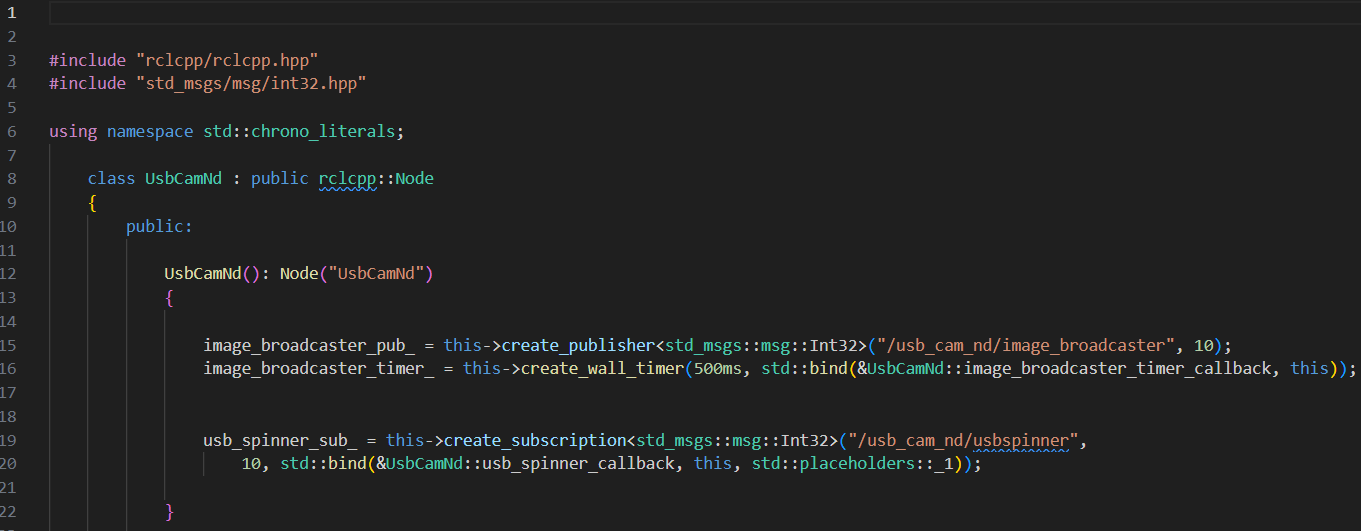
\includegraphics[width=\textwidth]{nocomment_example1.png}
	\caption{Example of generated code without comments}
	\label{figapp:nocomment_example1}
\end{figure}

When code comments are toggled on, the code from Figure~\ref{figapp:nocomment_example1} becomes the code from Figure~\ref{figapp:comment_example1}

\begin{figure}[htbp]
	\centering
	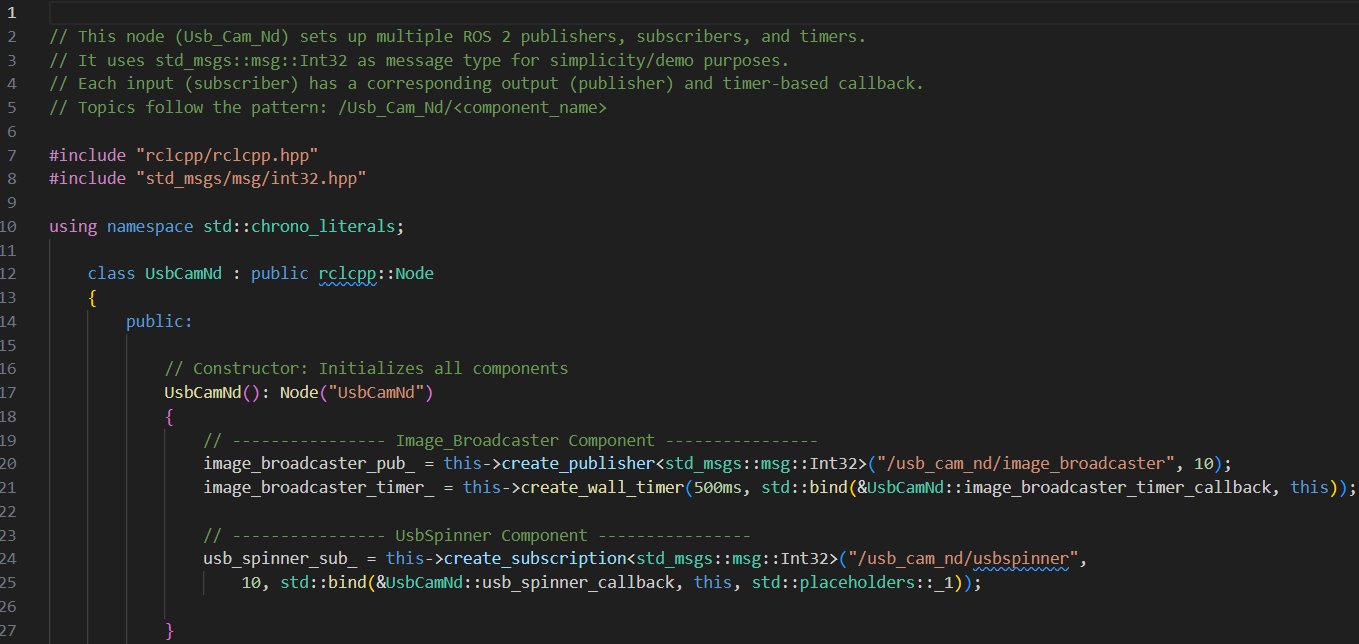
\includegraphics[width=\textwidth]{comment_example1.png}
	\caption{Example of generated code with comments}
	\label{figapp:comment_example1}
\end{figure}












